  \documentclass[12pt, a4paper, oneside]{article}\usepackage[]{graphicx}\usepackage[]{color}
%% maxwidth is the original width if it is less than linewidth
%% otherwise use linewidth (to make sure the graphics do not exceed the margin)
\makeatletter
\def\maxwidth{ %
  \ifdim\Gin@nat@width>\linewidth
    \linewidth
  \else
    \Gin@nat@width
  \fi
}
\makeatother

\definecolor{fgcolor}{rgb}{0.345, 0.345, 0.345}
\newcommand{\hlnum}[1]{\textcolor[rgb]{0.686,0.059,0.569}{#1}}%
\newcommand{\hlstr}[1]{\textcolor[rgb]{0.192,0.494,0.8}{#1}}%
\newcommand{\hlcom}[1]{\textcolor[rgb]{0.678,0.584,0.686}{\textit{#1}}}%
\newcommand{\hlopt}[1]{\textcolor[rgb]{0,0,0}{#1}}%
\newcommand{\hlstd}[1]{\textcolor[rgb]{0.345,0.345,0.345}{#1}}%
\newcommand{\hlkwa}[1]{\textcolor[rgb]{0.161,0.373,0.58}{\textbf{#1}}}%
\newcommand{\hlkwb}[1]{\textcolor[rgb]{0.69,0.353,0.396}{#1}}%
\newcommand{\hlkwc}[1]{\textcolor[rgb]{0.333,0.667,0.333}{#1}}%
\newcommand{\hlkwd}[1]{\textcolor[rgb]{0.737,0.353,0.396}{\textbf{#1}}}%

\usepackage{framed}
\makeatletter
\newenvironment{kframe}{%
 \def\at@end@of@kframe{}%
 \ifinner\ifhmode%
  \def\at@end@of@kframe{\end{minipage}}%
  \begin{minipage}{\columnwidth}%
 \fi\fi%
 \def\FrameCommand##1{\hskip\@totalleftmargin \hskip-\fboxsep
 \colorbox{shadecolor}{##1}\hskip-\fboxsep
     % There is no \\@totalrightmargin, so:
     \hskip-\linewidth \hskip-\@totalleftmargin \hskip\columnwidth}%
 \MakeFramed {\advance\hsize-\width
   \@totalleftmargin\z@ \linewidth\hsize
   \@setminipage}}%
 {\par\unskip\endMakeFramed%
 \at@end@of@kframe}
\makeatother

\definecolor{shadecolor}{rgb}{.97, .97, .97}
\definecolor{messagecolor}{rgb}{0, 0, 0}
\definecolor{warningcolor}{rgb}{1, 0, 1}
\definecolor{errorcolor}{rgb}{1, 0, 0}
\newenvironment{knitrout}{}{} % an empty environment to be redefined in TeX

\usepackage{alltt} % Paper size, default font size and one-sided paper
%\graphicspath{{./Figures/}} % Specifies the directory where pictures are stored
%\usepackage[dcucite]{harvard}
\usepackage{rotating}
\usepackage{tikz}
\usepackage{setspace}
\usepackage{framed}
\usepackage{pdflscape}
\usepackage[flushleft]{threeparttable}
\usepackage{multirow}
\usepackage[comma, sort&compress]{natbib}% Use the natbib reference package - read up on this to edit the reference style; if you want text (e.g. Smith et al., 2012) for the in-text references (instead of numbers), remove 'numbers' 
\usepackage{graphicx}
%\bibliographystyle{plainnat}
\bibliographystyle{agsm}
\usepackage[colorlinks = true, citecolor = blue, linkcolor = blue]{hyperref}
%\hypersetup{urlcolor=blue, colorlinks=true} % Colors hyperlinks in blue - change to black if annoying
%\renewcommand[\harvardurl]{URL: \url}
\IfFileExists{upquote.sty}{\usepackage{upquote}}{}
\begin{document}
\title{Introduction to Calculus}
\author{Rob Hayward}
\date{\today}
\maketitle
This is all about understanding instantantaneous rates of change or how fast something is moving at each moment. For example, to understand the speed that Usain Bolt is traveling as he runs 100 meters. This first section has been adapted from \href{https://www.khanacademy.org/math/calculus/differential-calculus/intro_differential_calc/v/newton-leibniz-and-usain-bolt}{Khan Academy} 
\cite{Khan1}.  Please take a look at the video for an expansion of these ideas. 

\vspace{5 mm}
\begin{tikzpicture}[xscale = 1, yscale = 1/10, scale = 0.8]
\draw [thick, <->] (0,100) -- (0,0) -- (10,0);
\draw [thin] (0,0) -- (9.58, 100);
\node [below left] at (9,0) {x = seconds};
\node [above, rotate = 90] at (0,95) {y = meters};
\draw [<->, blue] (0,0) to [out = 57, in = 232] (9.58, 100);
\node [below right] at (9.58, 100) {UB};
\end{tikzpicture}

The average speed over the whole 100  meters is $\frac{\Delta y}{\Delta x}$ where $\Delta y$ is the distance travelled and $\Delta x$ is the time.  Looking at the graph, the slope of the line connecting the origin with the UB point is the speed.  This is also called \emph{the rise over the run}.  In this case the distance is 100 meters and the time is 9.58 seconds.  Therefore the average speed for 100 meters is,  

$$\text{Average Speed} = \frac{100}{9.58} = 10.43\frac{m}{s}$$

However, it is not likely that Usain is able to run at a constant speed.  It is more probable that he takes some time to accelerate and that he may lose energy towards the end of the race. The blue line shows what may be a more accurate picture of the actual speed over the 100 meters course.  To find the \emph{instantaneous speed} means finding the slope of the blue line. This is the equivalent of drawing a tangent to the blue line.  

It means computing the following (adapted from \cite{Maths}).
\vspace{5 mm}
Where $f(x)$ is the function that describes the blue line and $h$ is a tiny increment, 
\vspace{5 mm}
$$\text{Instantaneous Speed} = \frac{f(x_0 + h) - f(x_0)}{(x_0 +h) - x_0} = \frac{(y_1 + h) - y_0}{h}$$

\vspace{5 mm}
The \emph{derivative} of $f(x)$, denoted as, 
\vspace{5 mm}
$$f'(x) \text{or} \frac{\mathrm d f}{\mathrm d x}(x_0) \text{or} \frac{\mathrm d y}{\mathrm dx} (x_0);$$ 
\vspace{5 mm}
is given by
\vspace{5 mm}
$$f'(x_0) = \lim_{h \to 0} \frac{f(x_0 +h) - f(x_0)}{h}$$
\vspace{5 mm}
For example, if $f(x) is y = x^2$,  there is the following plot

\begin{knitrout}
\definecolor{shadecolor}{rgb}{0.969, 0.969, 0.969}\color{fgcolor}

{\centering 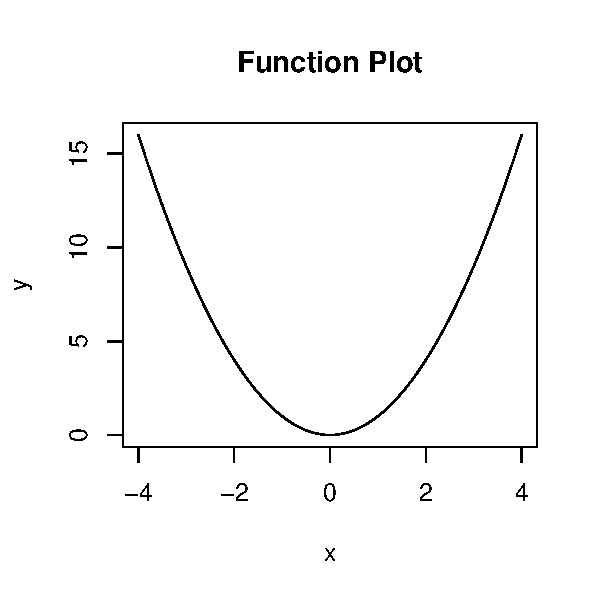
\includegraphics[width=\maxwidth]{figure/graph} 

}



\end{knitrout}


and the aim is to find the rate of change at the point (3, 9).

\vspace{5 mm}

\begin{centered}
\begin{tabular}{l r r r}
h & x + h & f(x + h) & $\frac{f(x +h) - f(x)}{h}\\
\hline
0.1 & 3.1 & 9.61 & 6.1 \\
0.01 & 3.01 & 9.0601 & 6.01 \\
0.001 & 3.001 & 9.0060 & 6.001\\
\end{tabular}
\end{centered}

\vspace{5 mm}
When $f(x) = x^2$, 

$$\frac{f(x_0 + h) - f(x_)}{h} = \frac{(x_0 + h)^2 - x_0^2}{h}$$
\vspace{5 mm}
$$\frac{x_0^2 +2x_0h + h^2 - x_0^2}{h} = \frac{h(2x_0 + h)}{h}$$
\vspace{5 mm}
$$2x + h$$

\begin{framed}
For integer k, the derivative of $f(x) = x^k$ at $x_0$ is $f'(x) = kx^{k-1}$.
\end{framed}
For example, the derivaitive of $f(x) = 2 + 3x + x^2$$ at $x_0$ is $f'(x) = 3 + 2x$$

Think about this. What determines the change at each value of x?  The 2 does not make any difference.  This just shifts the overall function up and down. On its own, $3x$ is a straight line.  We know that the gradient or slope is equal to 3. For $x^2$ the increase will be twice the value of $x$ (because it is squared).  

\section{Use of deriviatives}
Derivaitives can be very useful when looking at production and consumption decisions.  For example, with the following Total Physical Product function (TPP)

$$TPP = 100 +32Q + 10Q^2 - Q^3$$

It is possible to use the drivative to find the slope of the curve.  This would be the marginal physical product (MPP)


\begin{knitrout}
\definecolor{shadecolor}{rgb}{0.969, 0.969, 0.969}\color{fgcolor}
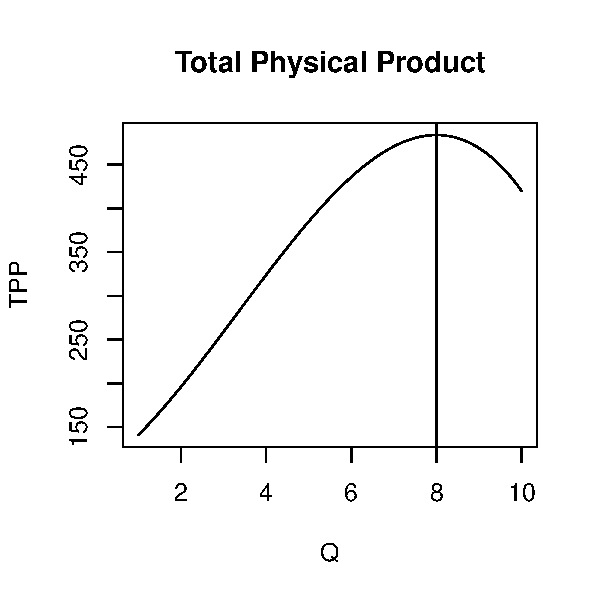
\includegraphics[width=\maxwidth]{figure/equation} 

\end{knitrout}


$$TTP' = MPP = 32 + 20Q - 3Q^2$

There is an example of this on page 138 of the textbook. 

\subsection{Maxima and Minima}
It can be useful to use derivatives to find maximum and minimum points.  At the maximum and at the mimimum the gradient will be equal to zero.  Therefore, to find the maximum or minimum, set the gradient to zero and solve. 
\vspace{5 mm}
For example, where is the maximum TPP in the previous example? 

As before, 

$$TTP' = MPP = 32 + 20Q - 3Q^2$

Set this equal to zero for a maximum, 

$$32 + 20Q - 3Q^2 = 0$$

or 

$$3Q^2 -20Q -32 = 0$$

There are two ways of solving this:
\begin{itemize}
\item Solving the equation
\item Trial and error
\end{itemize}e 

Solving equation requires finding the quadratic version of the equation.

So 

$$3Q^2 -20Q -32 = 0$$

Becomes

$$(3x + 4)(x - 8) = 0$$
\vspace{5 mm}
Therefore, $Q = -\frac{4}{3}$ or $Q = 8$
\vspace{5 mm}
Otherwise, plug in numbers until you reach the required.  The latter can be done particularly effectivley in excel (possibly with the solver application).  

\section{Application to Utility}
The same methods can be applied to questions about utility.  There is an example on page 66 of the textook repeated here \citep[p. 66]{Text}. 
\vspace{5 mm}
A utility function is described as 
\vspace{5 mm}
$$TU = 600Q - 4Q^2$$

\begin{knitrout}
\definecolor{shadecolor}{rgb}{0.969, 0.969, 0.969}\color{fgcolor}
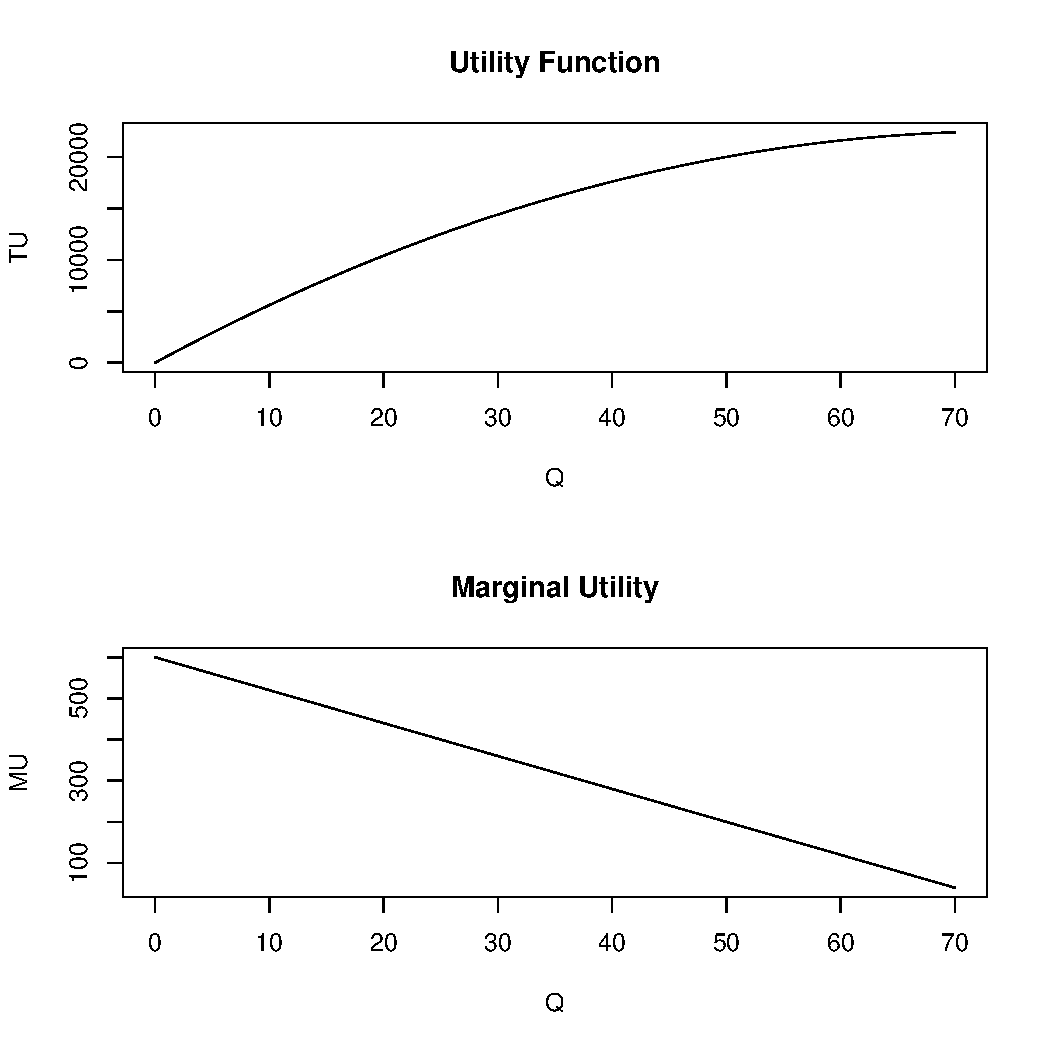
\includegraphics[width=\maxwidth]{figure/TU} 

\end{knitrout}

Where Q is the quantity of good consumed. The marginal utility would be the derivative of the total utility with respect to Q or, 
\vspace{5 mm}
$$ \frac{\mathrm d f}{\mathrm d Q}(600Q - 4Q^2) = 600 - 8Q$$



\bibliography{ref}
\end{document}
